\chapter{多相渗流模拟在GPU上的实现}
多孔介质内的多相流动是一类常见的复杂流动现象,在化石能源开采,化工过程,新能源等应用广泛。
目前LBM是模拟这类流动现象流行的数值方法,这得益于LBM在处理复杂流固边界和刻画多相多组分之间
相互作用的独特优势(见第\ref{chp:LBM}章)。但与上一章介绍的多孔介质内单相流动一样,在孔隙尺度
下直接运用LBM模拟多相渗流计算量通常相当大,一般需要利用并行计算加速。利用GPU加速LBM孔隙尺度
多相流计算目前在文献中报道较少,这也是本文工作的一个重点。
%ADD 前人在这方面工作相对较少。
本章讨论基于2.4节中多组分/多相模型的GPU实现。我们用两个算例验证了
多相流GPU程序实现的正确性,随后用其该模拟了二维和三维多孔介质中的两相流动,最后测试了其计算速度。
%ADD  上面的工作是否能完成

%%%%%%%%%%%%%%%%%%%%%%%%%%%%%%%%%%%%%%%%%%
\section{两组分LBM的GPU实现}
%多组分LBM与单组份LBM的GPU实现上有一些差异。
两组分LB模时,每个格点同时有两套PDF在演化,并且要考虑两组分间的相互作用对PDF变化的贡献。
就数据访问模式而言,每个格点除访问本身和周围格点的PDF外,还要访问其宏观量。在单组份情况
各个格点计算平衡态时只需要知道其本身的宏观量,即具有最理想的空间局部性,所以其计算过程
可以融合在计算迁移的Kernel中,也不需要为宏观量开辟存储空间,
但在两组分情况时,每个格点要访问周围格点的宏观量,若在碰撞迁移的Kernel中计算相邻格点的
宏观量显然进行大量的重复计算,因此我们采取的策略是为每个组分的宏观量$\rho_k$、$\bm u_k$
开辟全局内存,并另外增加一个Kernel\---\texttt{LBUpdateMacros},它在碰撞迁移的Kernel执行
完后统计每个组分的宏观量。

%%%%%%%%%%%%%%%%%%%%%%%%%%%%%%%%%%%%%%%%%%
\section{程序验证}
%%%%%%%%%%%%%%%%%%%%%%%%%%
\subsection{静止气泡测试} \label{subsec:bubble}
静止气泡测试可验证Laplace定律,是两相流中标准的模型验证算例之一。
Laplace定律给出了两相界面间压差$\Delta p$和界面表面张力$\gamma$之间的关系
\begin{equation}
  \Delta p = \sigma\frac{\gamma}{r}
  \label{laplace}
\end{equation}
对于二维情况$\sigma=1$,三维情况$\sigma=2$。对于球形界面$r$为球体半径,对于
圆柱形界面$r$为圆柱半径。

在进行静止气泡测试时,在计算区域中心球形区域内放置一种组分(即所谓的“气泡”),
球形区域以外放置另一种组分,待流场稳定后,压力场和气泡半径不再变化,如图\ref{fig:bubble}
所示。初始化流场时放置不同半径的气泡,稳定后得到不同的气泡半径$r_i$和界面压差$\Delta p_i$。
按照Laplace定律,$\Delta p_i$和$1/r_i$应该成正比。

这里指出,虽然我们编制的是D3Q19的GPU程序,但是为减少计算量,在实际计算时,
X方向只有一层格点,并且是周期边界,相当于计算的二维情况,后面的几个算例也是这种情况。

初始化时一个圆形状的组分被放在在YZ平面中心,平面四边均为周期边界,如图\ref{fig:bubble}所示。
%\begin{figure}[htb]
  %\centering
  %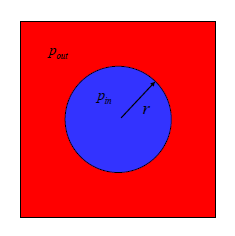
\includegraphics[]{img/bubble}
  %\caption{气泡示意图}
  %\label{fig:bubble}
%\end{figure}

\begin{figure}[htb]
  \centering
  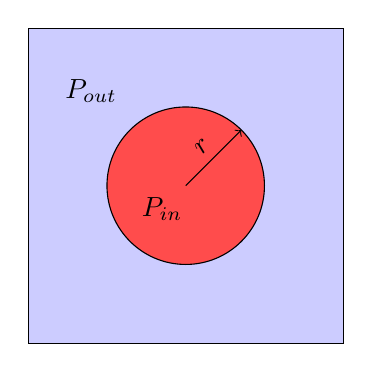
\begin{tikzpicture}
    \draw[fill=blue!20] (-2,-2) rectangle (2,2);
    \draw[fill=red!70] (0,0) circle (1);
    \draw (-0.3,-0.3) node[]{$P_{in}$};
    \draw (-1.2,1.2) node[]{$P_{out}$};
    \draw[->] (0,0) -- (0.707, 0.707) node[pos=0.5,sloped, above]{$r$};
  \end{tikzpicture}
  \caption{气泡示意图}
  \label{fig:bubble}
\end{figure}

%\begin{figure}[htb]
  %\centering
  %\subfigure[气泡示意图]{
    %\begin{minipage}[b]{0.4\textwidth}
      %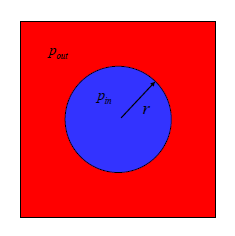
\includegraphics[width=1\textwidth]{img/bubble}
      %\label{fig:bubble}
    %\end{minipage}
  %}
  %\subfigure[测试结果]{
    %\begin{minipage}[b]{0.4\textwidth}
      %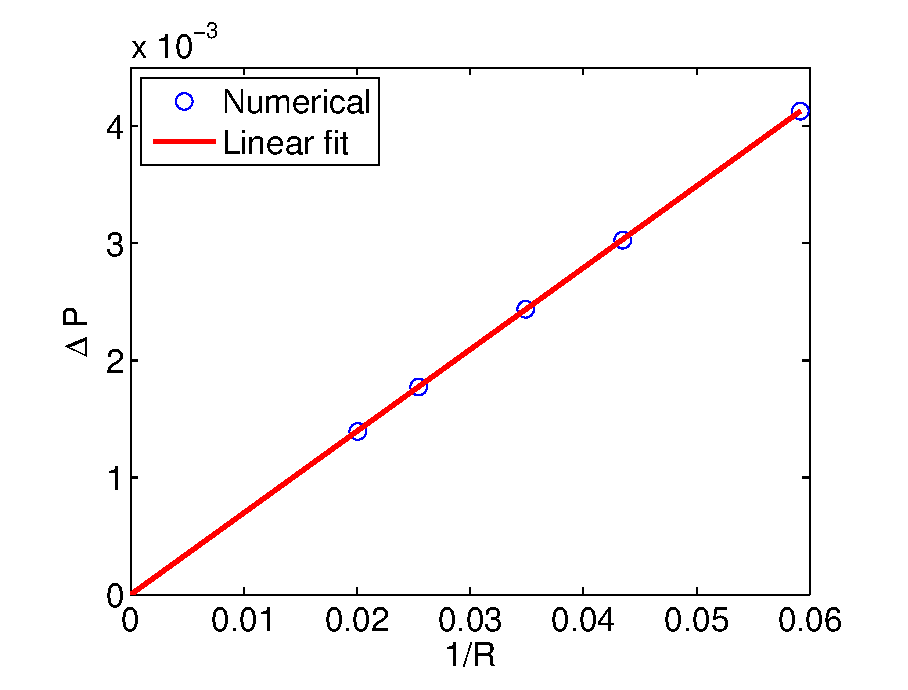
\includegraphics[width=1\textwidth]{img/bubble_test}
      %\label{fig:bubble_test}
    %\end{minipage}
  %}
  %\caption{气泡测试}
%\end{figure}

测试时两种流体粘性都为$1/6$,密度都为$1$,XY平面格点数为$128\times128$,
组分间相互作用系数$g_{k\bar k}=0.2$。
测试结果如图\ref{fig:bubble_test},可以看出计算结果与Laplace定律吻合良好。
\begin{figure}[htb]
  \centering
  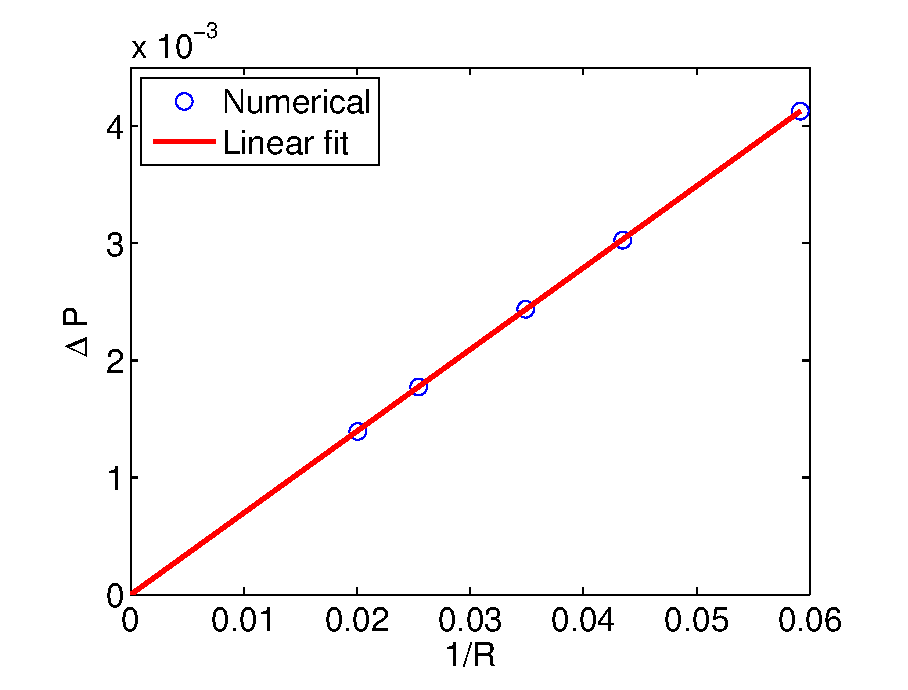
\includegraphics[width=0.6\textwidth]{img/bubble_test}
  \caption{气泡测试}
  \label{fig:bubble_test}
\end{figure}

%%%%%%%%%%%%%%%%%%%%%%%%%%
\subsection{层状两相流}
层状两相流如图\ref{fig:lcf}所示,在两块水平放置的平板间,两相流体在
沿X方向的外力驱动下一起向前运动。其中非润湿相处于中间层,厚度为$2a$,
而润湿相则贴近板壁,两板相距$2L$。两相流体受到的外力可以不同,分别为
$F_w$和$F_n$,下标$n$和$w$表示润湿相(wetting phase)和非润湿相(no wetting
phase)。
两相流体X方向速度在沿Y方向分布的解析解为\ucite{porter2012multicomponent}
\begin{subequations}\label{lcf_ana}
  \begin{flalign}
    u(y)=\frac{F_n}{2\nu_n\rho_n}(a^2-y^2)+\frac{F_w}{2\nu_w\rho_w}(L^2-a^2),
    \quad 0\leqslant |y|\leqslant a \\
    u(y)=\frac{F_w}{2\nu_w\rho_w}(L^2-y^2), \quad a \leqslant |y| \leqslant L
  \end{flalign}
\end{subequations}
\begin{figure}[htb]
  \centering
  \begin{tikzpicture}[scale = 1.5]
    \draw[fill=blue!20] (-3,-1) rectangle (3,1);
    \draw[dashed, fill=red!70] (-3,-0.5) rectangle (3,0.5);
    \draw[very thick](-3, 1) -- (3,1);
    \draw[very thick](-3, -1) -- (3,-1);

    \draw[dashed, thick](-3.2, 0) -- (3.2,0);

    \draw (-2,0.75) node[] { 润湿相};
    \draw (-2,-0.25) node[] {非润湿相};

    \draw[->, thick] (0, 0.75) node[left] {$\bm  F_w$} -- (0.5, 0.75);
    \draw[->, thick] (0, -0.25) node[left] {$\bm  F_n$} -- (0.5, -0.25);
    \draw[->] (-2.5, 1.3) node[left]{平板} -- (-2, 1.05);
    \draw[<->] (2.6, 0) -- node[left]{$a$}  (2.6, 0.5);

    \draw (3, 1) -- (3.15, 1);
    \draw[<->] (3.1, 0) -- node[right]{$L$}  (3.1, 1.0);
  \end{tikzpicture}
  
  \caption{层状两相流示意图}
  \label{fig:lcf}
\end{figure}

%\begin{figure}[htb]
  %\centering
  %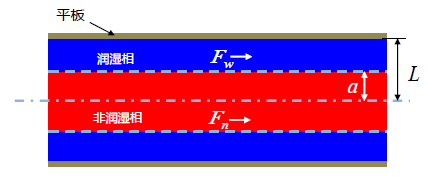
\includegraphics[]{img/lcf}
  %\caption{层状两相流示意图}
  %\label{fig:lcf}
%\end{figure}

算例中设置的计算参数为$\rho_n=\rho_w=1.0$,$\nu_w=10/6,\nu_n=1/6$,
$F_n=F_w=1.0\time10^{-6}$,组分间作用系数$g_{k\bar k}=0.27$,Y方向
网格个数为256。计算结果与解析解的对比如图\ref{fig:lcf_vx_a}所示,可以
发现二者吻合良好。
\begin{figure}[htb]
  \centering
  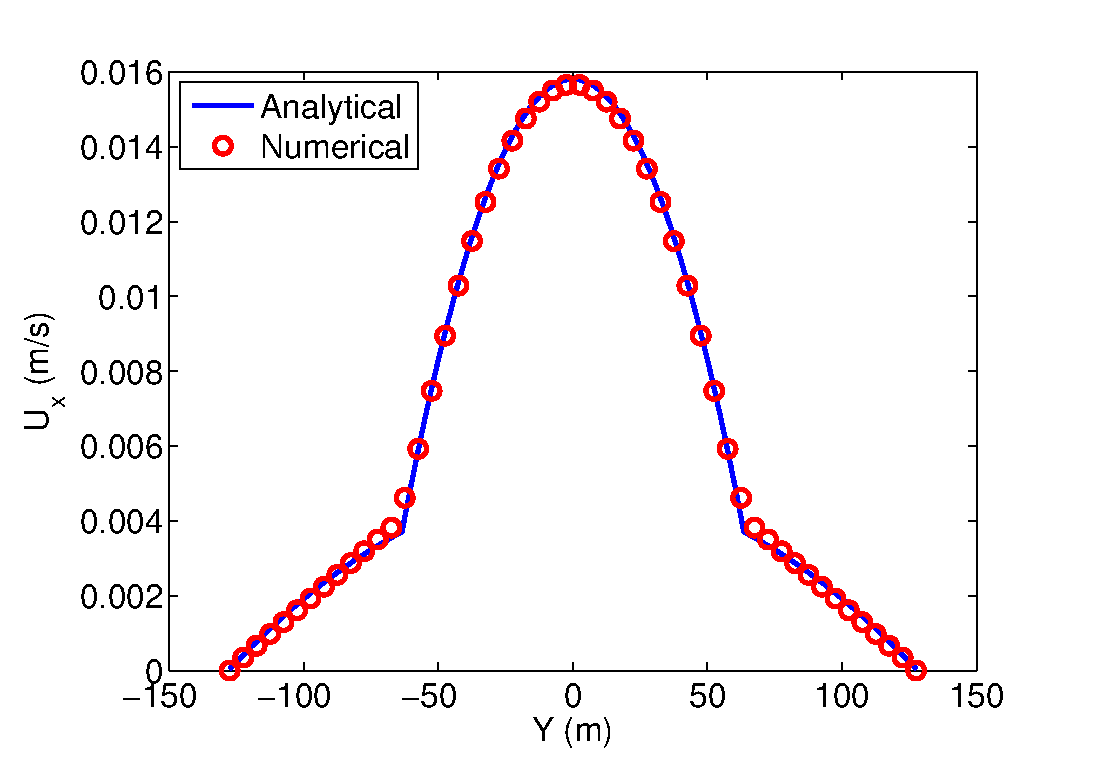
\includegraphics[width=0.6\textwidth]{img/lcf_vx_a}
  \caption{沿Y方向的速度分布}
  \label{fig:lcf_vx_a}
\end{figure}

%%%%%%%%%%%%%%%%%%%%%%%%%%
\subsection{液滴测试}
为验证润湿性边界条件处理的正确性,我们进行了液滴测试,并获得了组分
固体表面间相互作用强度与接触角的关系。组分与固体表面的接触角反应了两种
组分对固体表面的相对润湿性。在Shan-Chen模型(或我们所使用的改进模型)
中,接触角大小主要取决于两种流体组分(组分g与f)与固体表面(s)
间相互作用强度系数$G_{gs}$、$G_{gs}$以及组分间相互作用强度系数$G_{fg}$。
另外,$G_{fg}$大小影响相界面厚度和数值稳定性,我们发现$G_{fg}=0.2$时比较
理想,所以接下来的测试中取$G_{fg}=0.2$。

计算开始时,在一个长$800$高$200$的二维长管道的下底板放置一个半径为$50$半圆形组分
f,其他区域分布着另一组分g,管道左右边界是周期边界,上下边界是固壁,
示意图见图\ref{fig:droplet}。
%\begin{figure}[htb]
  %\centering
  %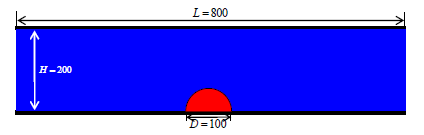
\includegraphics[]{img/droplet}
  %\caption{液滴示意图}
  %\label{fig:droplet}
%\end{figure}

\begin{figure}[htb]
  \centering
   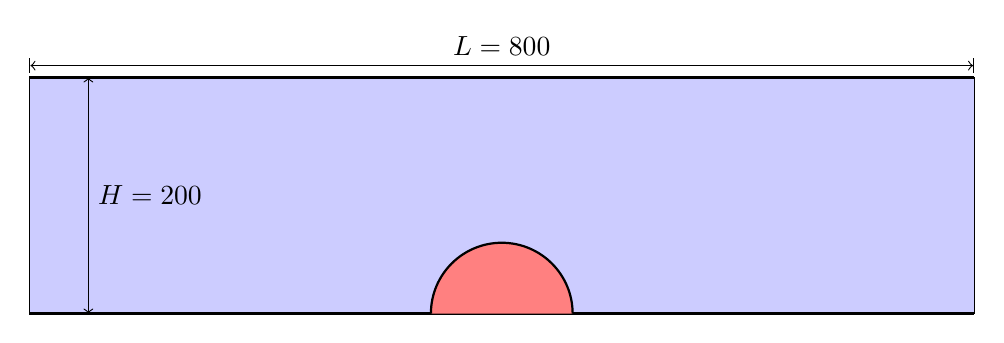
\begin{tikzpicture}[scale = 1.5]
    \draw[fill=blue!20] (-4, 0) rectangle (4,2);
    \draw[<->] (-3.5, 0) -- node[right]{$H=200$} (-3.5, 2);
    \draw[very thick] (-4, 2) -- (4, 2);
    \draw[very thick] (-4, 0) -- (4, 0);
    \draw[|<->|] (-4, 2.1) -- node[above]{$L=800$} (4, 2.1);
    %\draw[fill=red!50] (0:0.5) -- arc (0:180:0.5);
    \draw[thick, fill=red!50] (0:0.6) arc (0:180:0.6);
  \end{tikzpicture}
  \caption{液滴示意图}
  \label{fig:droplet}
\end{figure}
通过调整$G_{fs}$、$G_{gs}$的取值,液滴会呈现不同接触角,计算结果见图
\ref{fig:drop_A}至图\ref{fig:drop_G}。
每幅图只画出了液滴附近的区域。

\begin{figure}[htb]
  \centering
  \subfigure[$G_{fs}=-0.005, G_{gs}=0.005$]{
    \begin{minipage}[b]{0.4\textwidth}
      
\includegraphics[width=0.8\textwidth]{img/drop_img/drop_A}
      \label{fig:drop_A}
    \end{minipage}
  }
  \subfigure[$G_{fs}=0.0, G_{gs}=0.0$]{
    \begin{minipage}[b]{0.4\textwidth}
      
\includegraphics[width=0.8\textwidth]{img/drop_img/drop_E}
      \label{fig:drop_E}
    \end{minipage}
  }
  \\
  \subfigure[$G_{fs}=-0.01, G_{gs}=0.01$]{
    \begin{minipage}[b]{0.4\textwidth}
      
\includegraphics[width=0.8\textwidth]{img/drop_img/drop_B}
      \label{fig:drop_B}
    \end{minipage}
  }
  \subfigure[$G_{fs}=0.01, G_{gs}=-0.01$]{
    \begin{minipage}[b]{0.4\textwidth}
      
\includegraphics[width=0.8\textwidth]{img/drop_img/drop_F}
      \label{fig:drop_F}
    \end{minipage}
  }
  \\
  \subfigure[$G_{fs}=-0.02, G_{gs}=0.02$]{
    \begin{minipage}[b]{0.4\textwidth}
      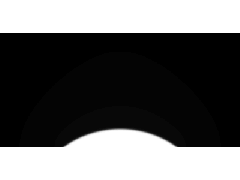
\includegraphics[width=0.8\textwidth]{img/drop_img/drop_C}
      \label{fig:drop_C}
    \end{minipage}
  }
  \subfigure[$G_{fs}=0.02, G_{gs}=-0.02$]{
    \begin{minipage}[b]{0.4\textwidth}
      
\includegraphics[width=0.8\textwidth]{img/drop_img/drop_G}
      \label{fig:drop_G}
    \end{minipage}
  }
  \\
  \subfigure[$G_{fs}=-0.03, G_{gs}=0.03$]{
    \begin{minipage}[b]{0.4\textwidth}
      
\includegraphics[width=0.8\textwidth]{img/drop_img/drop_D}
      \label{fig:drop_D}
    \end{minipage}
  }
  \subfigure[$G_{fs}=0.03, G_{gs}=-0.03$]{
    \begin{minipage}[b]{0.4\textwidth}
      
\includegraphics[width=0.8\textwidth]{img/drop_img/drop_H}
      \label{fig:drop_H}
    \end{minipage}
  }
  \caption{接触角测试结果}
\end{figure}

%%%%%%%%%%%%%%%%%%%%%%%%%%%%%%%%%%%%%%%%%%
\section{多相渗流模拟}
在上一节中的验证算例中,流固边界相对简单,我们在这一节中
计算了实际多孔介质中的二维和三维两相渗流。
%%%%%%%%%%%%%%%%%%%%%%%%%%%%%%%%%%
\subsection{二维多相渗流模拟}
计算过程使用的二维多孔介质如图\ref{fig:porousMedid2D}所示,
图中黑色区域为固体,白色部分为孔隙,前处理时将其离散为$802\times478$
的个格子大小。初始化时,在孔隙中随机布满两种纯组分,即每个孔隙格点
以相同的概率被设为组分f或g。两种组分粘性为$\nu_f=\nu_g=1/6$,密度
为$\rho_f=\rho_g=1$。流体在向右的大小为$F=10^{-4}$的外力驱动下运动。
组分间相互作用强度为$G_{gf}=0.15$, 组分与固壁间的相互作用强度分别为
$G_{fs}=0.03,G_{gs}=-0.03$,根据上一节液滴测试的结果,在这组参数下,
组分f形成的相是非润湿相,而组分g形成的相是润湿相,并且非润湿相
接触角接近$180^o$。
%布满两种流体组分$f$和$g$,
\begin{figure}[htb]
  \centering
  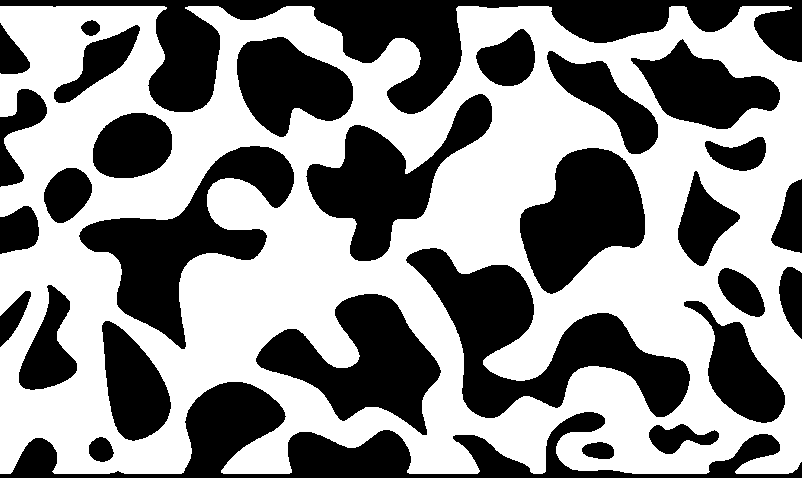
\includegraphics[width=0.6\textwidth]{img/porousMedia2D}
  \caption{二维多孔介质结构}
  \label{fig:porousMedid2D}
\end{figure}
图\ref{fig:porousMedid2D_A}至\ref{fig:porousMedid2D_E}所示为不同演化步
时两相的分布,其中红色部分为润湿相(组分g),蓝色部分为非润湿相(组分f)。
可以发现在流动过程中润湿相包围着固壁,而非润湿相则被润湿相包围,这是
多相渗流基本的现象。
\begin{figure}[htb]
  \centering
  \subfigure[第1000步]{
    \begin{minipage}[b]{0.4\textwidth}
      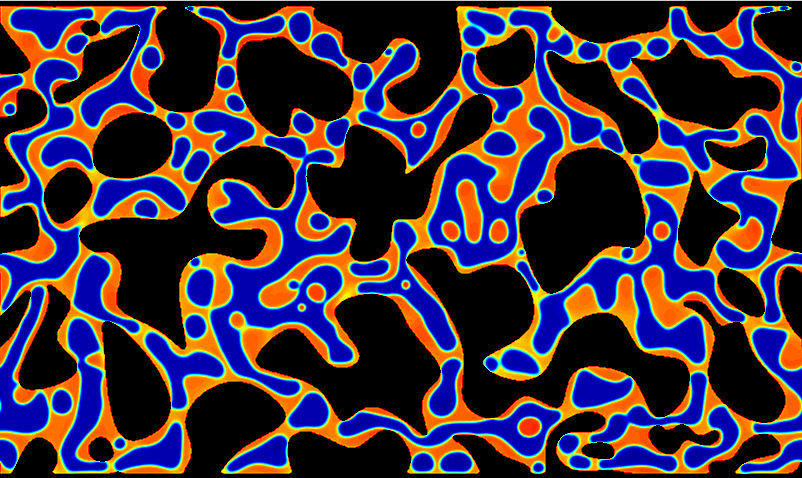
\includegraphics[width=0.8\textwidth]{img/open/GG_00001000}
      \label{fig:porousMedid2D_A}
    \end{minipage}
  }
  \subfigure[第5000步]{
    \begin{minipage}[b]{0.4\textwidth}
      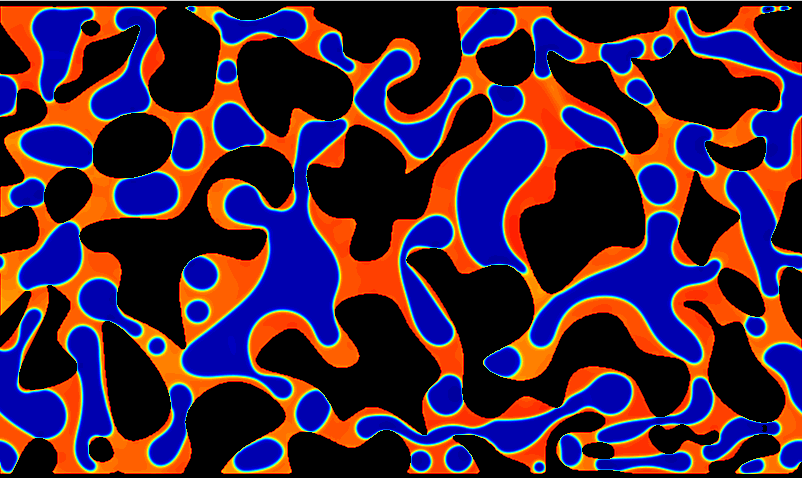
\includegraphics[width=0.8\textwidth]{img/open/GG_00005000}
      \label{fig:porousMedid2D_B}
    \end{minipage}
  }
  \\
  \subfigure[第10000步]{
    \begin{minipage}[b]{0.4\textwidth}
      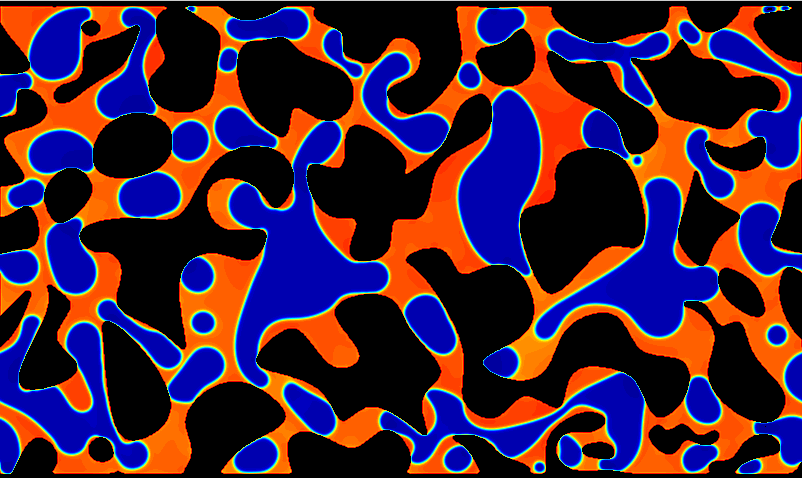
\includegraphics[width=0.8\textwidth]{img/open/GG_00010000}
      \label{fig:porousMedid2D_C}
    \end{minipage}
  }
  \subfigure[第20000步]{
    \begin{minipage}[b]{0.4\textwidth}
      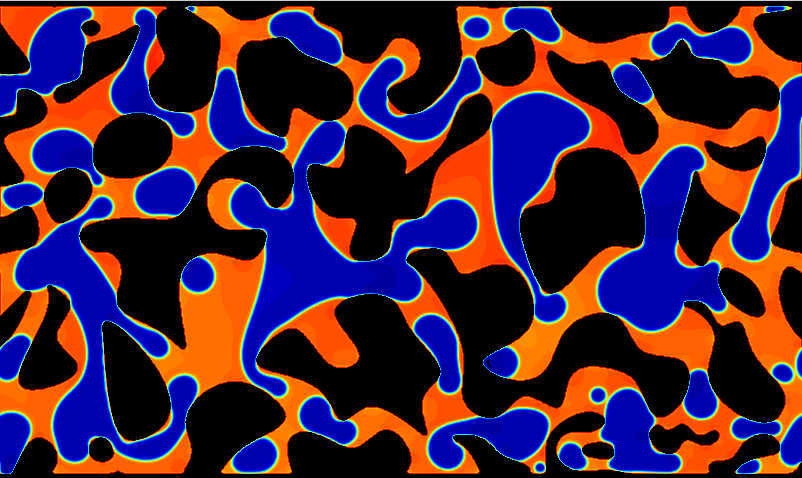
\includegraphics[width=0.8\textwidth]{img/open/GG_00020000}
      \label{fig:porousMedid2D_D}
    \end{minipage}
  }
  \\
  \subfigure[第30000步]{
    \begin{minipage}[b]{0.4\textwidth}
      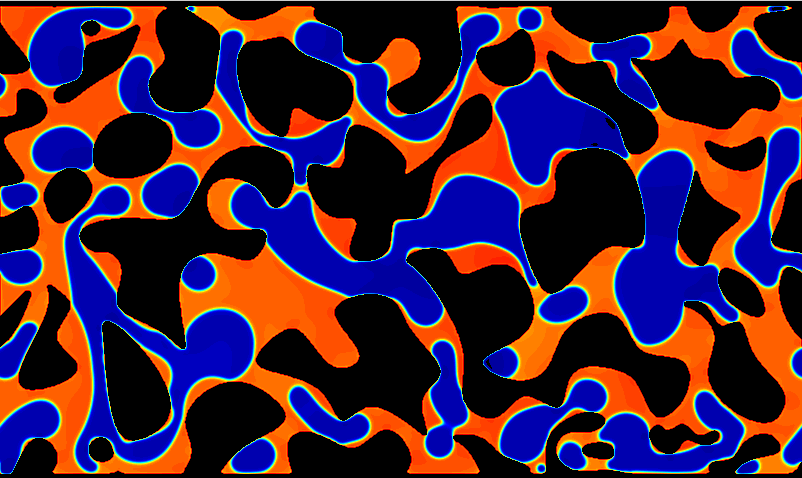
\includegraphics[width=0.8\textwidth]{img/open/GG_00030000}
      \label{fig:porousMedid2D_E}
    \end{minipage}
  }
  \subfigure[第40000步]{
    \begin{minipage}[b]{0.4\textwidth}
      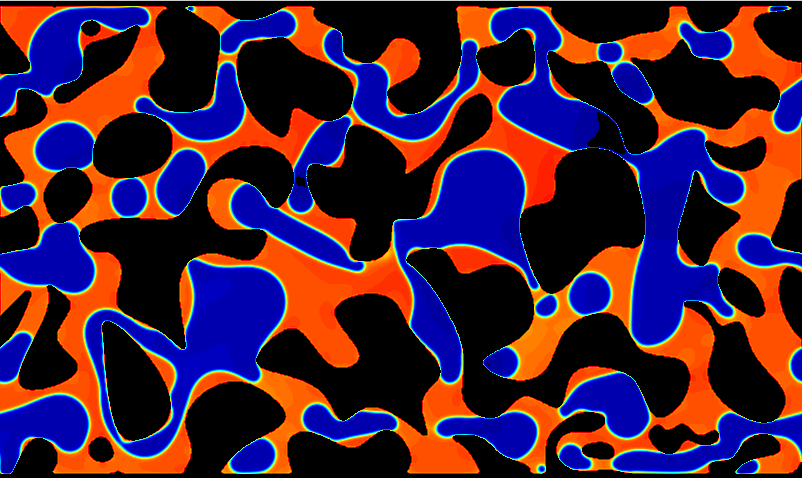
\includegraphics[width=0.8\textwidth]{img/open/GG_00040000}
      \label{fig:porousMedid2D_F}
    \end{minipage}
  }
  \caption{二维多相渗流模拟}
\end{figure}

%%%%%%%%%%%%%%%%%%%%%%%%%%%%%%%%%%

\subsection{三维维多相渗流模拟}
这一节中我们模拟了一种人工生成的多孔介质内的两相流,该多孔介质由
大小和位置随机分布的球体堆积而成,其孔隙结构如图\ref{fig:balls}所示,
其孔隙率大小为0.7。各个面均为周期性边界条件,初始化时孔隙内各格点
按相等概率随机给定组分f或组分g。流体受沿X方向的外力驱动。
演化100000步时,流场内部两相分布如图\ref{fig:3d_porous_2_phase}所示,
其中蓝色部分为固体区域,红色部分为非润湿相,绿色部分为润湿相。

\begin{figure}[htpb]
  \centering
  \subfigure[随机球体堆积多孔介质模型]{
    \begin{minipage}[b]{0.4\textwidth}
      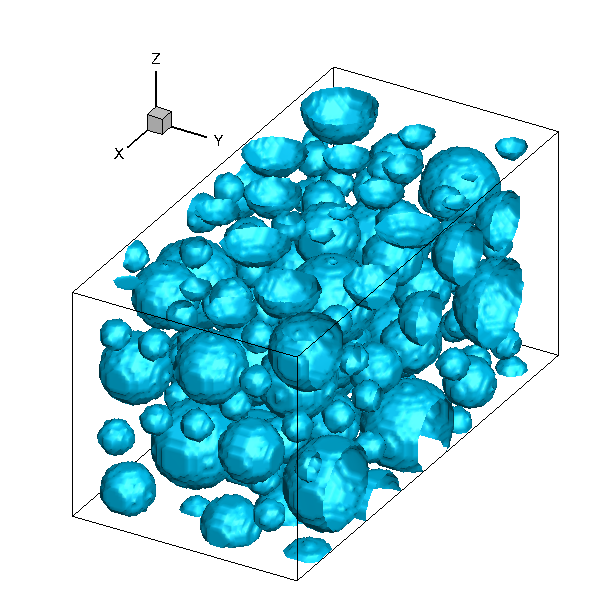
\includegraphics[width=0.9\textwidth]{img/3d_porous/balls}
      \label{fig:balls}
    \end{minipage}
  }
  \subfigure[演化100000步时两相分布]{
    \begin{minipage}[b]{0.4\textwidth}
      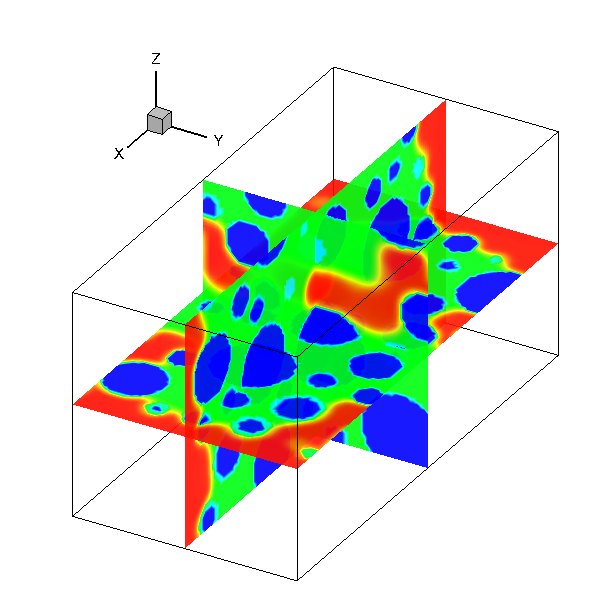
\includegraphics[width = 0.9\textwidth]{img/3d_porous/2_phase}
      \label{fig:3d_porous_2_phase}
    \end{minipage}
  }
  \caption{三维多孔介质两相流}
\end{figure}


\section{性能测试}
\subsection{性能测试}
\subsubsection{性能预测}
%多相流计算程序相对于单相流计算程序在算
我们根据上一章中单组分流动稀疏存储算法GPU程序性能来预测本章多组分模拟GPU程序性能,二者在计算上的区别有如下几点:
\begin{itemize}
  \item 两组分程序中每个格点存储两套PDF,并且碰撞前需要访问相邻格点宏观量,访存量增加
    超过1倍;
  \item 两组分程序碰撞前需要计算组分间相互作用,计算量增大;
  \item 两组分程序中多了一个\texttt{LBUpdateMacros} Kernel函数;
  \item 两组分程序需特殊处理流固边界(润湿性边界),引入线程判断和分支;
\end{itemize}
考虑到LB的GPU计算性能瓶颈在访存带宽,所以上述几个因素中第一个因素对性能影响最大,即两组分相对单组份性能至少下降
一半。
另外我们运用CUDA工具箱中的Visual Profiler 分析发现\texttt{LBUpdateMacros} Kernel函数占整个演化过程计算时间的22\%左右。
综合上述因素我们预测两组分相对单组份计算速度下降70\%左右。上一章中采用稀疏存储算法的单组分计算GPU程序的流体格点更新速率为
210MFLUPS左右(单精度,见图\ref{fig:speed_algo_MFL}),因此我们预测本章的两组分计算程序速度大概为60MLUPS。

\subsubsection{网格数的影响}
我们分别测试了二维和三维流场在不同网格数下的计算速度,流场中不含固体格点(即Kernel中没有判断分支),二维和
三维计算采用的是同一个程序,二维情况只算一层流体格点(见\ref{subsec:bubble}小节解释)。采用单精度计算时,
速度测试结果如图\ref{fig:chp6_speed_2d}和\ref{fig:chp6_speed_3d}所示。
可以发现二维和三维情况计算速度均为70MLUPS左右,三维情况最高速度可达80MLUPS。
\begin{figure}[htpb]
  \centering
  \subfigure[二维]{
    \begin{minipage}[b]{0.4\textwidth}
      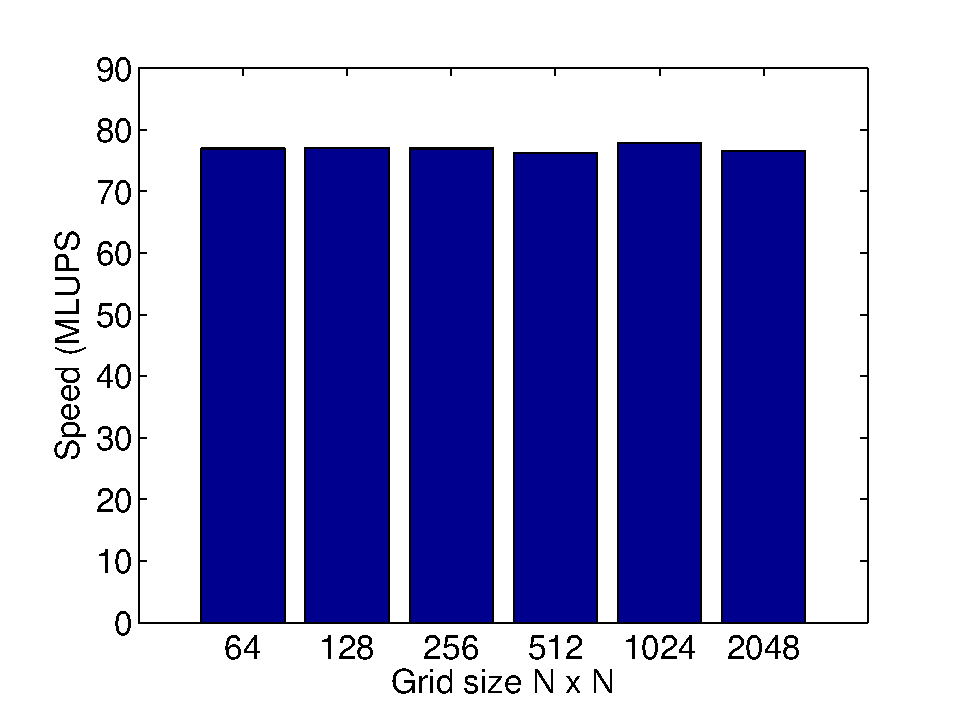
\includegraphics[width=0.9\textwidth]{img/chp6_speed_2d}
      \label{fig:chp6_speed_2d}
    \end{minipage}
  }
  \subfigure[三维]{
    \begin{minipage}[b]{0.4\textwidth}
      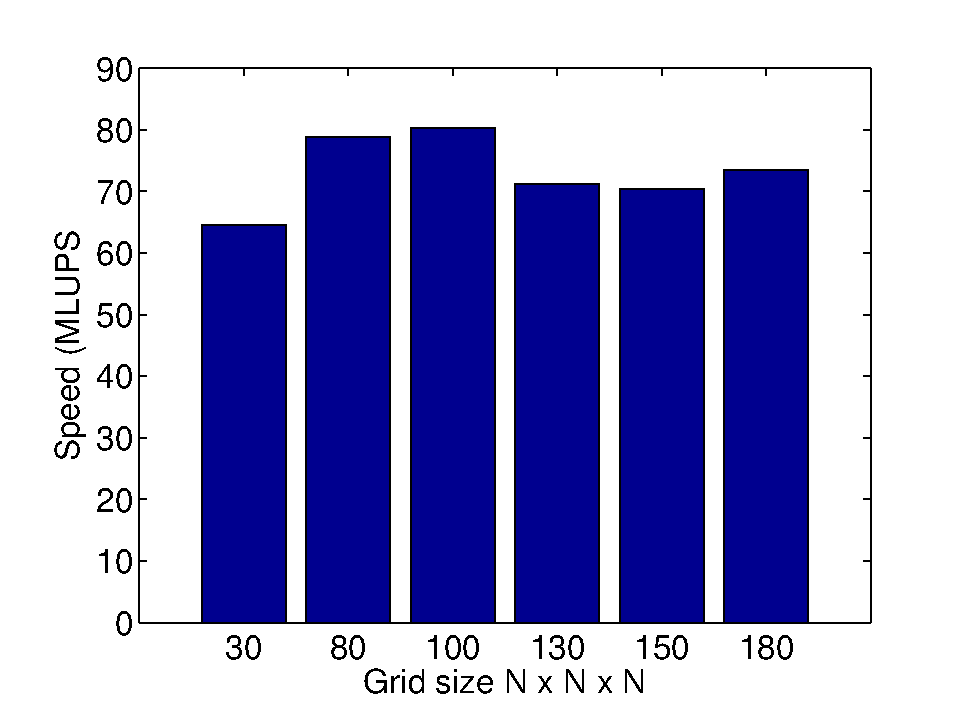
\includegraphics[width=0.9\textwidth]{img/chp6_speed_3d}
      \label{fig:chp6_speed_3d}
    \end{minipage}
  }
  \caption{网格数对计算速度的影响}
\end{figure}

\subsubsection{流固边界的影响}
因为Kernel函数中处理流固边界润湿性时引入了分支判断语句,对GPU程序执行效率会有影响。
我们测试在不同复杂程度的流场时的计算速度,所用三种流场如图\ref{fig:chp6_A}至\ref{fig:chp6_C}所示。
图\ref{fig:chp6_A}为最简单的情形,没有固体格点;图\ref{fig:chp6_B}所示为上一节中使用的随机球体
多孔介质模型,其流场较为复杂;图\ref{fig:chp6_C}为随机生成的方块填充多孔介质结构,其流场
结构最为复杂。
\begin{figure}[htpb]
  \centering
  \subfigure[没有固体格点]{
    \begin{minipage}[b]{0.3\textwidth}
      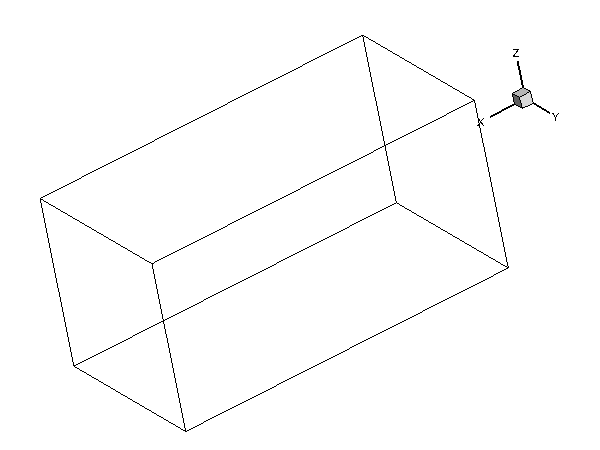
\includegraphics[width=0.9\textwidth]{img/3d_porous/A}
      \label{fig:chp6_A}
    \end{minipage}
  }
  \subfigure[随机球体]{
    \begin{minipage}[b]{0.3\textwidth}
      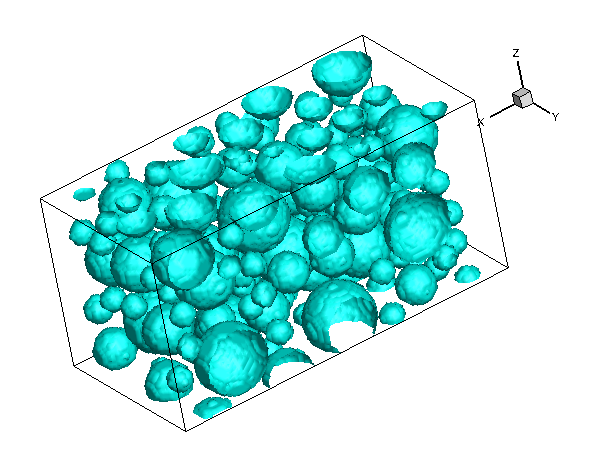
\includegraphics[width=0.9\textwidth]{img/3d_porous/B}
      \label{fig:chp6_B}
    \end{minipage}
  }
  \subfigure[随机方块]{
    \begin{minipage}[b]{0.3\textwidth}
      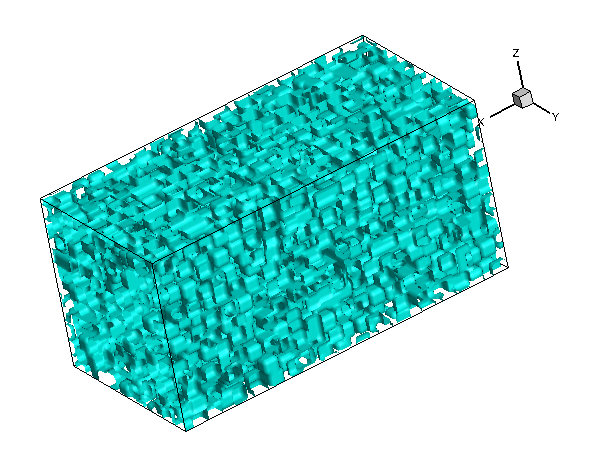
\includegraphics[width=0.9\textwidth]{img/3d_porous/C}
      \label{fig:chp6_C}
    \end{minipage}
  }
  \caption{不同复杂程度的流场结构}
\end{figure}

三种情况网格数均为$64\times 64 \times 128$,速度测试结果如图\ref{fig:chp6_speed_ABC}所示。
可以发现流场结构越复杂,计算速度越慢,最复杂的情况相对最简单的情况计算速度下降33\%。
\begin{figure}[htb]
  \centering
  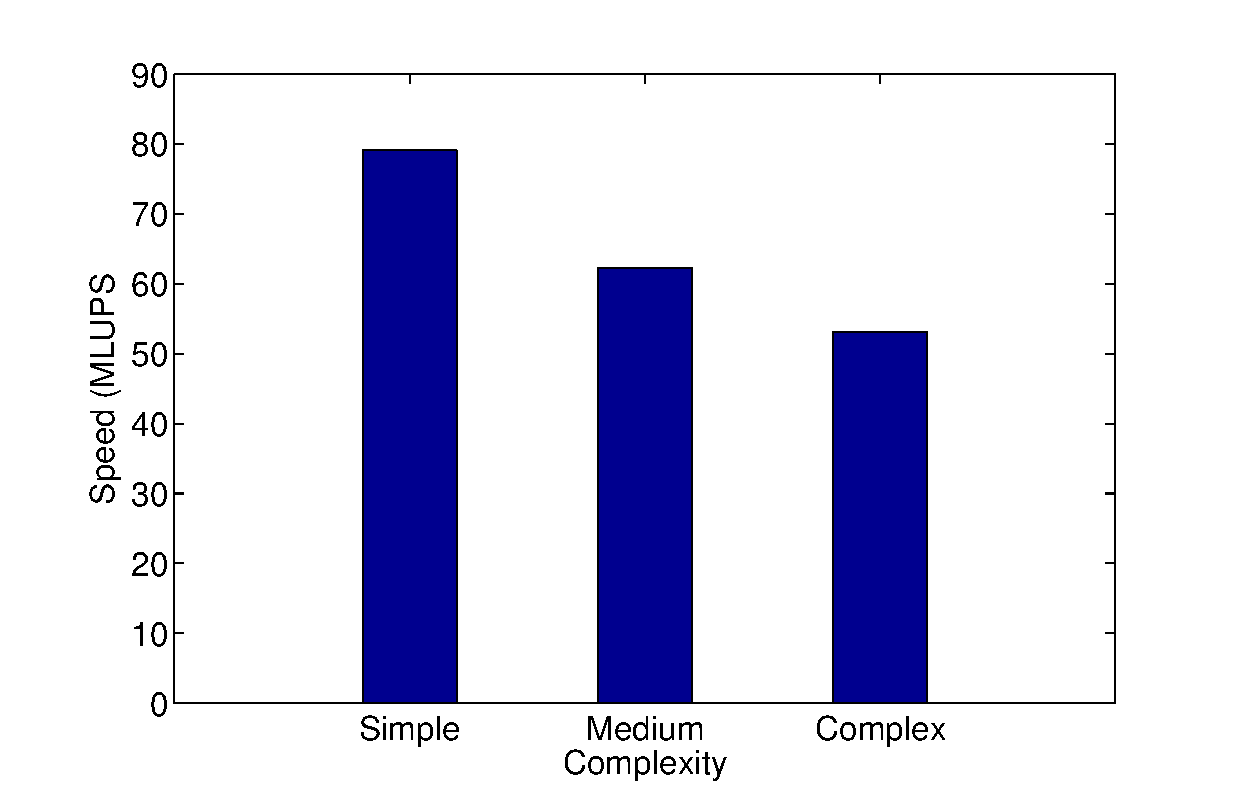
\includegraphics[width=0.6\textwidth]{img/chp6_speed_ABC}
  \caption{流场复杂程度对计算速度的影响}
  \label{fig:chp6_speed_ABC}
\end{figure}

%\subsection{程序结构}
%本节简介本本研究过程中针对多孔介质中单相/多相流所开发的GPU计算程序。

%根据前面章节介绍的系数存储模式,首先要根据表示多孔介质结构的\texttt{flag}数组
%重构格点的之间的连接关系。我们将这一过程与计算过程分开处理,作为前处理过程。

\section{小结}
本章介绍了两相渗流LB模拟在GPU上的实现。
针对多组分LB模型在GPU上实现时的难点我们重新设计了演化的Kernel函数,
并增加了一个Kernel单独计算宏观量。
我们首先通过气泡测试、层状两相流、接触角测试验证了我们程序实现的正确性,
随后分别模拟了二维和三维的两相渗流,计算结果显示的流动现象与实际情况相符。
最后进行了程序性能测试,并分析了影响计算速度的因素,发现我们的两组分GPU程序
的最高计算速度可达80MFLUPS,而我们计算相同问题的CPU版本程序速度最快为1.96MFLUPS,
因此GPU加速比超过40。

